% !TeX root = ../main.tex
% Add the above to each chapter to make compiling the PDF easier in some editors.


\chapter{Introduction}\label{chapter:introduction}

Curiosity is one of our main drives. Even in babies the desire to model the world helps them endure many of the difficulties of exploring it. A baby might stumble, fall, get burnt or scratched but still will continue to be relentlessly curious trying to construct a useful model of the world. An important part of this model is understanding and recognizing other people. This is due to the fact that humans are fundamentally social animals. Our ability to communicate with each other in a sophisticated way sets us apart from all other animals. The first step of this communication occurs before we even open our mouths when we recognize each other physically, gauge each others posture, and detect other non-verbal clues. Recognizing other people enables us to respond to each others actions, cooperate or compete with each other. This is so central to our lives that it is unimaginable to operate in a world without this ability. 

The ability to perform spatial reasoning of objects and people in a scene is crucial for performing any complex function. Recognizing human posture and motion is equally if not more important for robots which inhabit the same physical space with us. This makes it a critical problem for Computer Vision and Robotics. The long held vision where we have robots in our houses assisting in housework, cleaning, and cooking even helping us take care of our elderly all need this ability to function properly.

Additionally, as the aspect of having artificially intelligent agents becomes more realistic we discover many more applications where recognizing human pose is an urgent necessity. Autonomously driving cars need to recognize the actions of pedestrians around them in order to operate intelligently. Many autonomous driving systems require the driver to be alert while the car is driving itself. Monitoring the driver and controlling his alertness and health is also important. Robots working in a manufacturing plant hand in hand with people need to accurately detect and recognize the body posture and motion of people around them. There are also many practical applications which would benefit from such a technology such as virtual and augmented reality. This shows again that artificial intelligence systems which depend on human interactions in a physical medium need to have Human Pose Estimation as part of their system.

Our body conveys a lot of information about our actions and well being as well. There are so many subtle clues from the way we sit to the pace of our walk about our personality and health. Our posture can give clues about our level of confidence, whether we cross our arms or show our hands sends signals that we are protective or open in a given situation. Our body also gives many signals relating to our health through our motions. Many illnesses relating to balance can be recognised by analyzing the way a person walks. Many of our insights also depend on our ability to measure and record them. Recognizing the human body in a computational medium opens up a whole new area of applications. Having large scale accurate quantitative metrics about human motion is posed to give rise to advances in our understanding about human motion which can be useful in sports analysis, kinematic modeling in animation and robotics. 

In this thesis we focused on developing a human pose estimation system in clinical gate analysis. Gate analysis is a fundamental technique for diagnosing vertigo and balance disorders. Many illnesses originating from disorders relating to brain,ear,eye dysfunction or psychological disorders can manifest themselves in a person's gait. Reaching a diagnosis in balance related illnesses is difficult and requires a variety of tests ranging from video oculography to gait analysis. It has been shown that gait deficits during dual-task walking are important markers for the cognitive development of patients and for tracking of dimensia realted disorders \parencite{schniepp2016erfassung}. Some critical and fatal conditions like brain strokes can also be observed through a gait test. This makes the availability of this kind of diagnosis tools important.

The dataset that we developed our application for was created by the administration of a gait analysis test in the German Center for Vertigo and Balance Disorders (DSGZ) during its regular operation over 11 years. The test consisted of 8 tasks which where usually repeated a few times. In each task the patient would walk on the GAITRite(R) pressure carpet performing a certain action. Actions include, self-paced walk, slow walk, fast walk, walking with eyes closed, walking with a reclined head, walking while making calculations and walking while doing a verbal task. The GAITRite(R) carpet is collecting gait statistics like stride length, stride width and stride frequency. These statistics are normalized with respect to age and gender. The resulting data is reported based on how many standard deviations the statistics are apart when compared to measurements from an age-matched healthy control group. The deviations are expressed as a so-called z-matrix, where each column corresponds to a measurement and each row to a task. An example of a Z-Matrix can be seen below. From now on we will refer to this dataset as the gait dataset.

The gait dataset consist of both gait statistics calculated from the pressure carpet and a web-cam footage of the gait sequence. Our aim in this thesis was to utilize the monocular video data to estimate the gait parameters. The gait footage is captured from roughly the direction of the pressure carpet. This makes the distance estimation and therefore the gait statistics calculations a significant problem. An example of the footage can be seen in \autoref{fig:gait-footage}

\begin{figure}[htpb]
	\centering
	\begin{subfigure}[b]{0.3\linewidth}
   		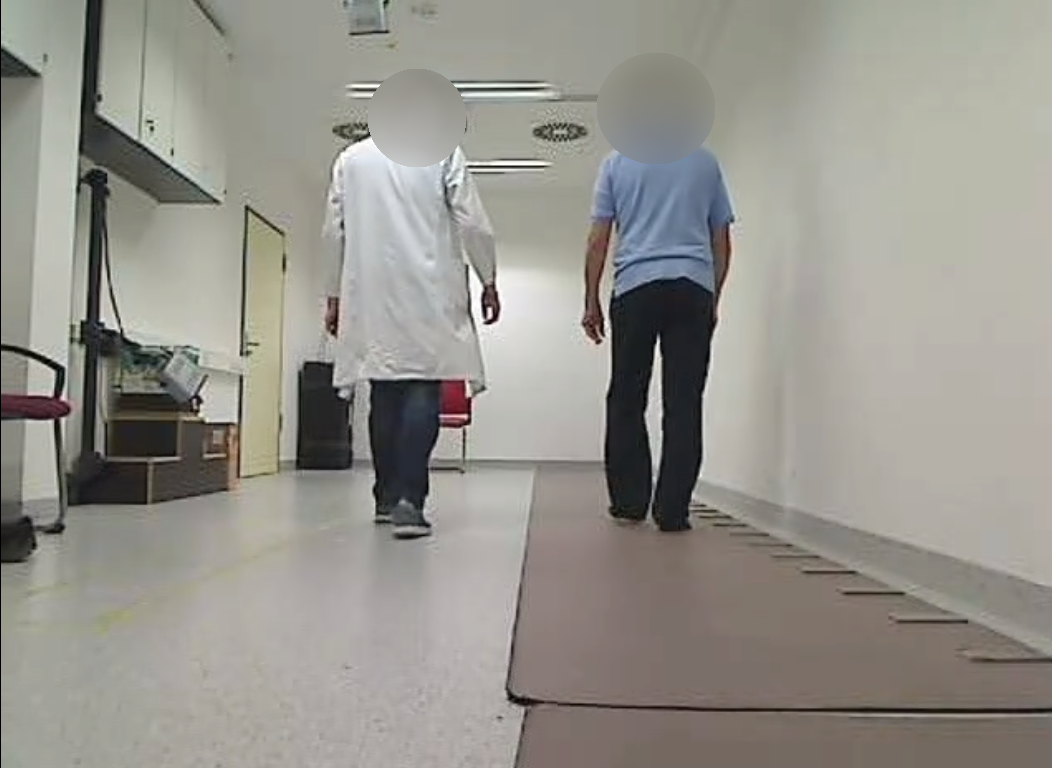
\includegraphics[width=\linewidth]{gp2.png}
    	\caption{Walking Away from the camera}
    \end{subfigure}
    \begin{subfigure}[b]{0.3\linewidth}
   		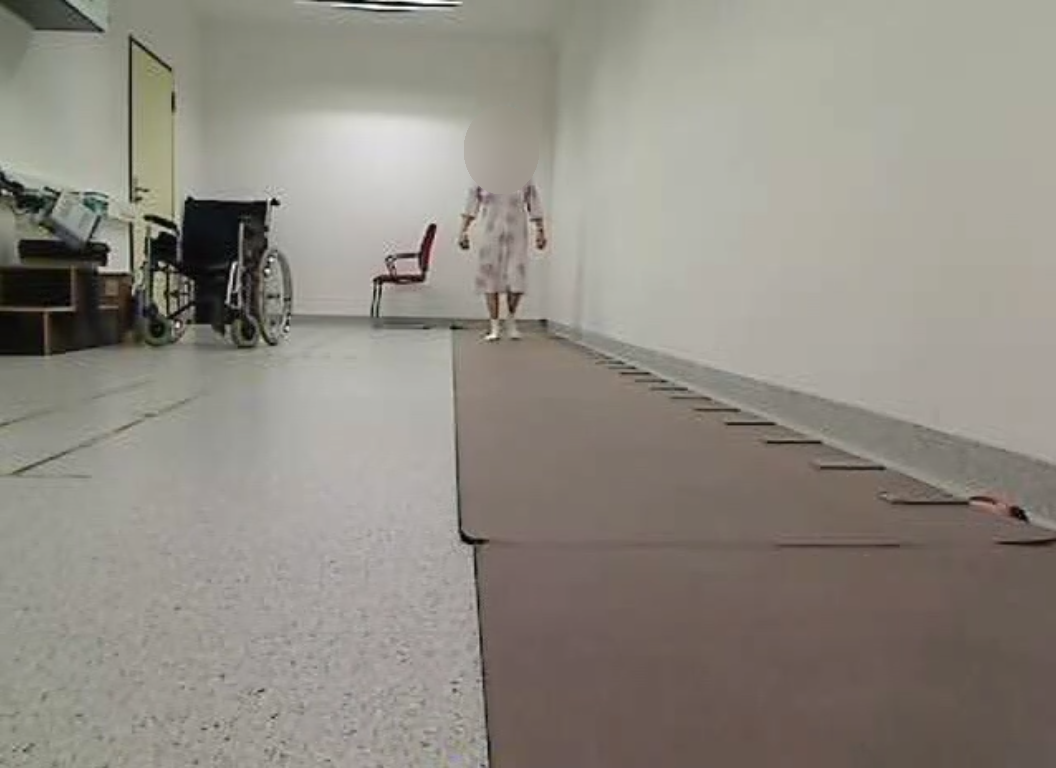
\includegraphics[width=\linewidth]{gp13.png}
    	\caption{Walking towards the camera}
    \end{subfigure}
    \begin{subfigure}[b]{0.3\linewidth}
   		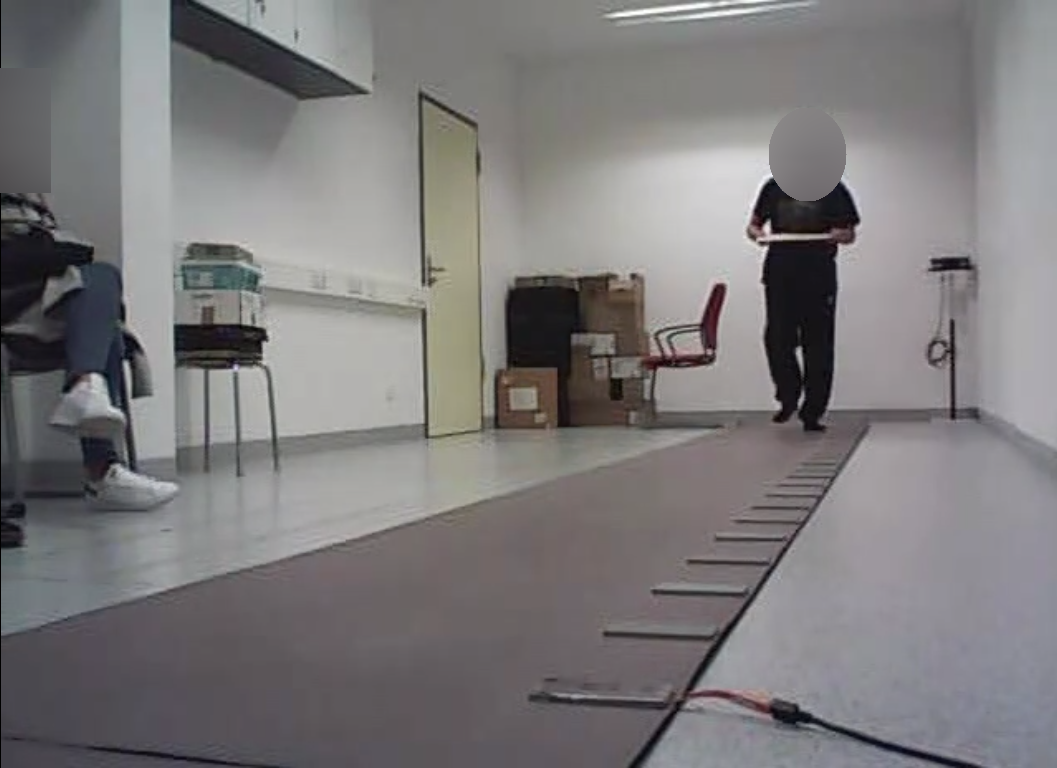
\includegraphics[width=\linewidth]{gp17.png}
    	\caption{Walking while holding a tray}
    \end{subfigure}
    \caption{Example frames from the gait dataset}
    \label{fig:gait-footage}
\end{figure}

There has been many deep learning based successful 2D pose estimation techniques in recent years that work in challenging everyday settings \parencite{newell2016stacked}, \parencite{chu2017multi}, \parencite{chou2017self} ,some even in multi person pose estimation scenarios \parencite{cao2016realtime}, \parencite{iqbal2017posetrack}, \parencite{insafutdinov2017arttrack}. The availability of large annotated datasets played an important role in advancing this field. However, 2D poses are inherently ambiguous because an arbitrary camera viewpoint can make totally different poses look similar or some body part or objects can occlude the view from others. To illustrate one can think of a scenario where whether the person is facing towards or away from the camera cannot be determined just by looking at a 2D projection. Look at \autoref{fig:ambiguity} for an example. Although, 3D pose estimation doesn't suffer from these shortcomings it is a more difficult problem. Mainly, obtaining large quantities of annotated 3D poses requires a motion capture setup which is difficult and costly to setup and the visual data in the laboratory setup is very constraint. In order to make a successful pose estimation, a model has to be invariant to a number of factors like background scenes, lighting, clothing shape and texture, skin color and image imperfection. Models trained on these datasets have a hard time generalizing to in-the-wild scenarios.

\begin{figure}[htpb]
    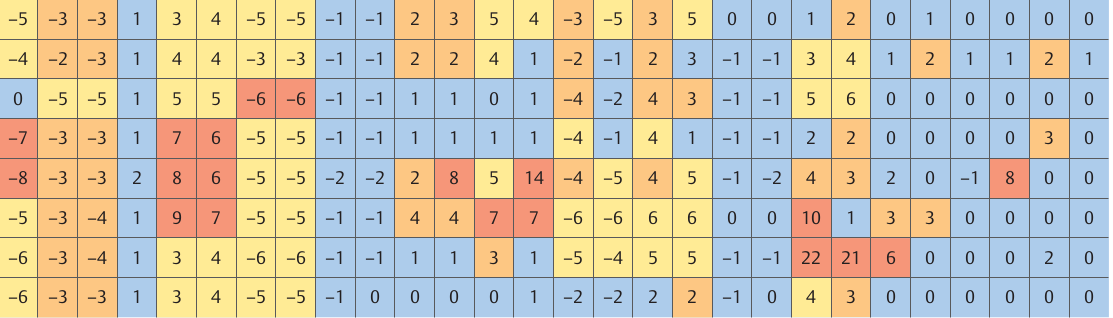
\includegraphics[width=\linewidth]{zmatrix.png}
    \caption{Image showing ambiguity in the 3D pose}
    \label{fig:ambiguity}
\end{figure}

Our approach is to decouple the problem of 3D pose estimation from a monocular image to 2D pose estimation from monocular image and lifting the pose from 2D to 3D. This approach has several advantages. 
\begin{itemize}
    \item Firstly, 2D pose estimation methods like \parencite{cao2016realtime} perform very well on in-the-wild scenarios where there exists large annotated datasets like MPII \parencite{andriluka20142d} and MS-COCO \parencite{lin2014microsoft}. This enables us to perform high quality 2D pose estimations from gait sequence videos.
    \item Secondly, it is possible to train a 2D to 3D pose estimator for arbitrary camera viewpoints and distances. This is accomplished through projecting the 3D annotated joint positions to the required camera positions.
    \item Thirdly, this makes the problem remarkably simpler and allows for a greater range of solutions to be explored.
\end{itemize}

In order to estimate the gait parameters we used \parencite{cao2016realtime}'s pose estimator to obtain 2D pose sequences. This method was the best performing multi person pose estimation methods available. These formed the fundamental building block for the remaining models. We trained several 2D-3D pose estimators to obtain accurate 3D poses from different viewpoints and distances. One first model is using feed forward network with residual connections in a frame by frame basis. The second model is exploiting temporal information by using a synchronized sequence to sequence network. The third model is using additional height information together with a loss function which preserves the lengths of the bones. We train models for both 3D to Z-matrix estimation and 2D to Z-matrix estimation and compared the results.

There are several contributions of this work. First we train a network which estimates 3D human pose from different viewpoints and distances. This enables us to estimate 3d human poses in in-the-wild  scenarios which was not possible with previous methods. Secondly we show that exploiting both  temporal information and skeletal structural priors improves pose estimation results significantly. Lastly we use our last model to infer 3D pose from our gait data and estimated their corresponding z-matrices.

\section{Problem Definition}

The main problem we are trying to solve is estimating z-matrix values for the videos in the gait dataset. This requires multi-step pipeline to accomplish. First, given a monocular low resolution 350x600 gait video infer 2D pixel location sequence of 14 joints depicted in \autoref{fig:joints2D}. Secondly, given the 14 joint pixel positions infer 3D position sequence of those joints. Lastly, given 3D position sequence for a gait video estimate gait parameters in terms of a z-matrix row.

\begin{figure}[htpb]
    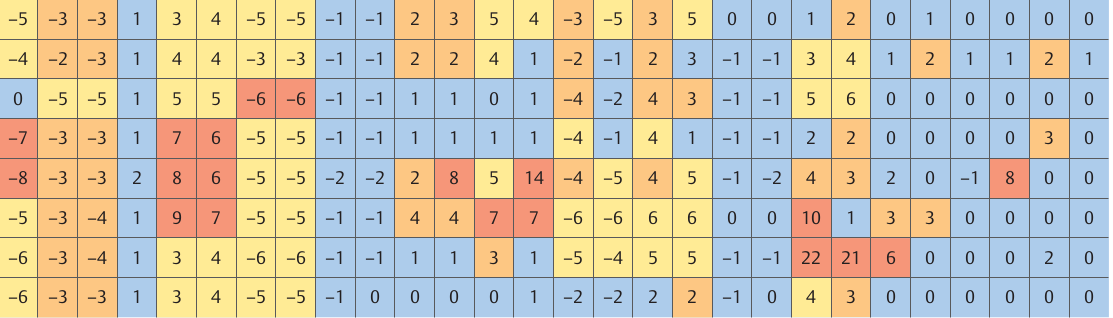
\includegraphics[width=\linewidth]{zmatrix.png}
    \caption{Illustration of the detected joints in the human body}
    \label{fig:joints2D}
\end{figure}

There are several considerations that need to be regarded when designing a solution for this problem. 
\begin{itemize}
    \item The gait videos can sometime contain together with the person who is taking the gait test an administrator who is standing next to the patient or sitting in the other side of the room. See \autoref{fig:gait-problems} (a) and (c)
    \item Portions of the body of the subject is not visible in the beginning or end of videos due to the placement of the camera. \autoref{fig:gait-problems} (b) and (e)
    \item All joints can not be detected in all frames. For example, when the patient is walking away from the camera the nose joint can not be detected throughout the video. See \autoref{fig:gait-problems} (a)
    \item The viewing angles of the training datasets and camera positioning of the gait videos are drastically different. See \autoref{fig:gait-problems} (a) and (b)
    \item During the gait videos the patient is walking either towards or away from the camera. This forces the model to be invariant to different distances. See \autoref{fig:gait-problems} (e) and (f)
    \item The patients have different heights and body compositions. This constitutes another source of ambiguity, since it is not clear given a 2D projection whether the person is tall and farther away from the camera or small and close to the camera. See \autoref{fig:gait-problems} (a) and (f)
\end{itemize}

\begin{figure}[htpb]
	\centering
	\begin{subfigure}[b]{0.3\linewidth}
   		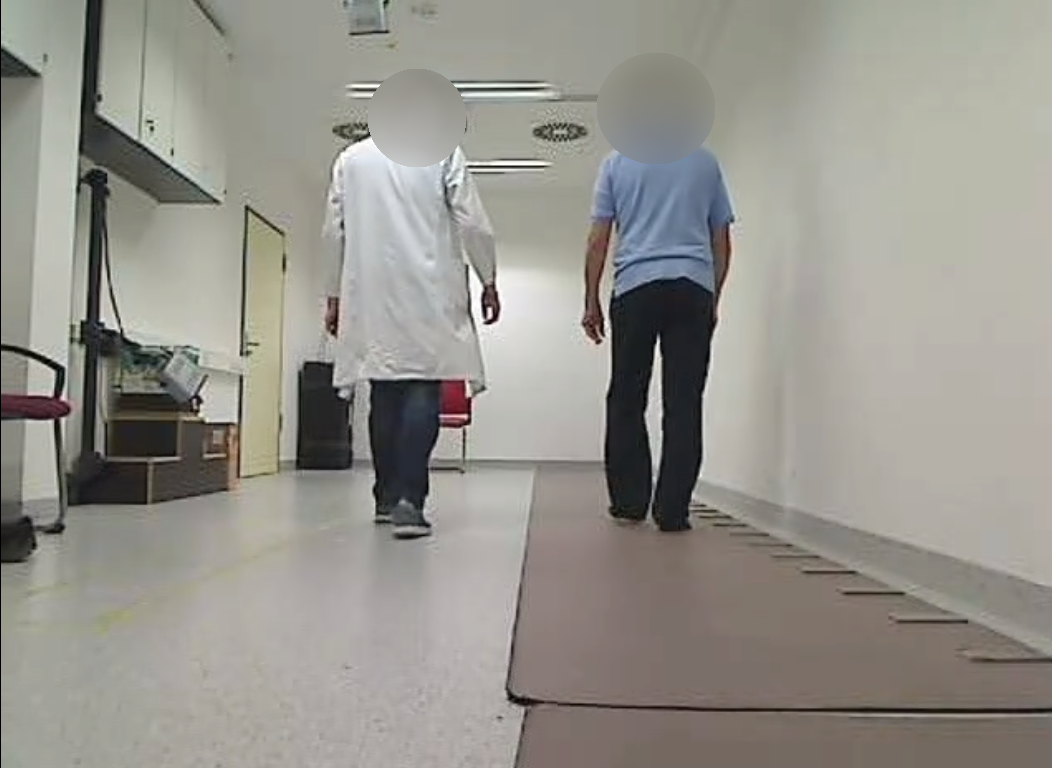
\includegraphics[width=\linewidth]{gp2.png}
    	\caption{Two People in Scene}
    \end{subfigure}
    \begin{subfigure}[b]{0.3\linewidth}
   		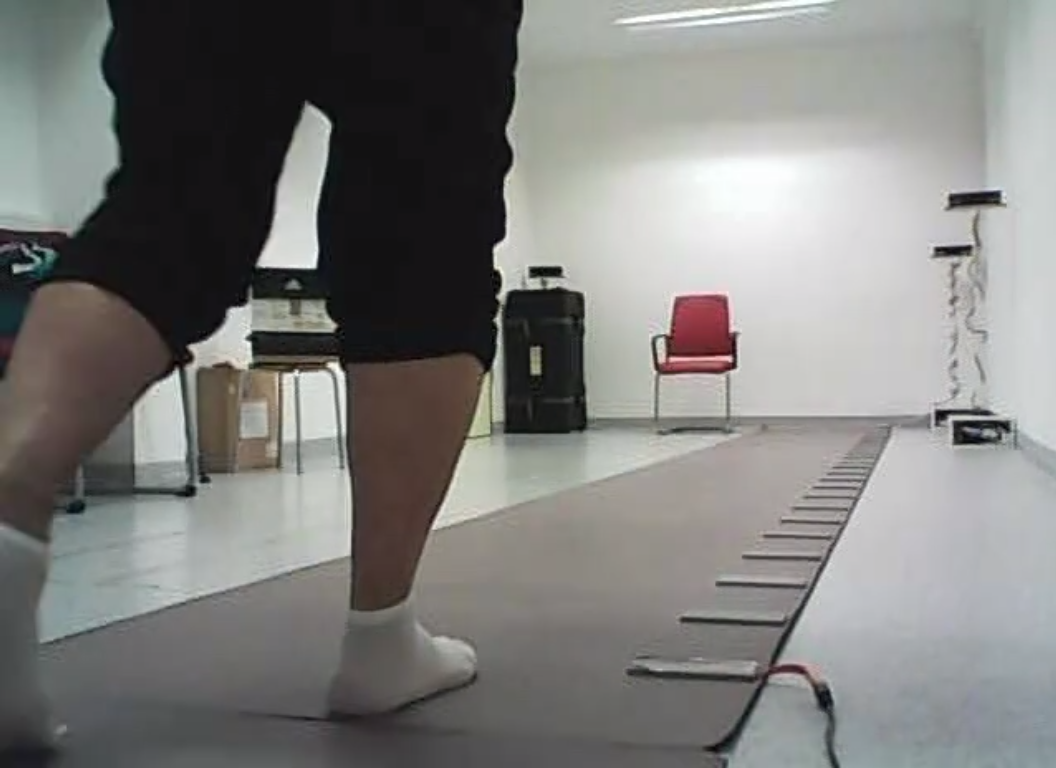
\includegraphics[width=\linewidth]{gp4.png}
    	\caption{Out of camera view}
    \end{subfigure}
    \begin{subfigure}[b]{0.3\linewidth}
   		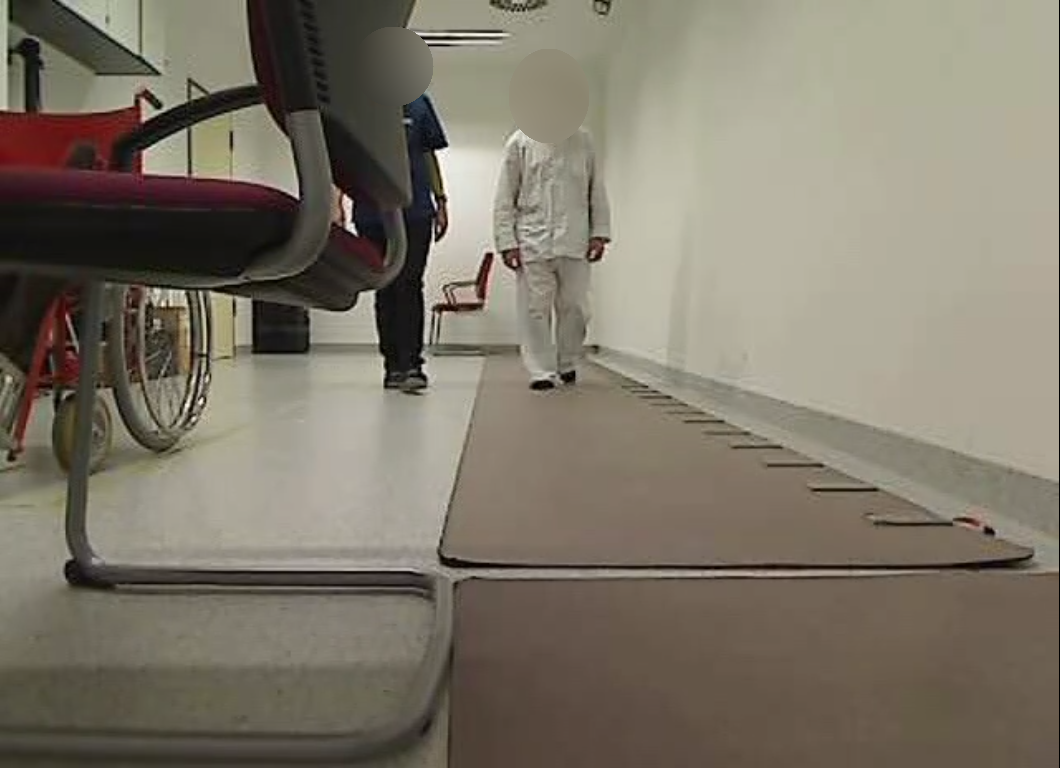
\includegraphics[width=\linewidth]{gp6.png}
    	\caption{Obscured view}
    \end{subfigure}
    \begin{subfigure}[b]{0.3\linewidth}
   		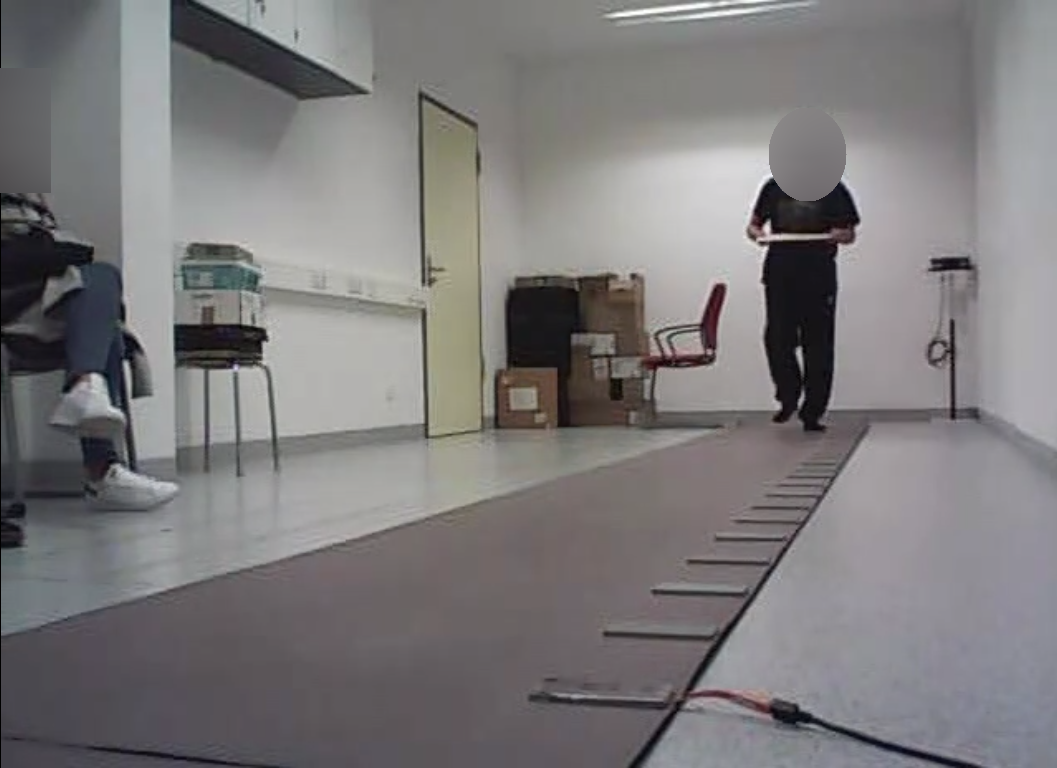
\includegraphics[width=\linewidth]{gp17.png}
    	\caption{Person sitting}
    \end{subfigure}
    \begin{subfigure}[b]{0.3\linewidth}
   		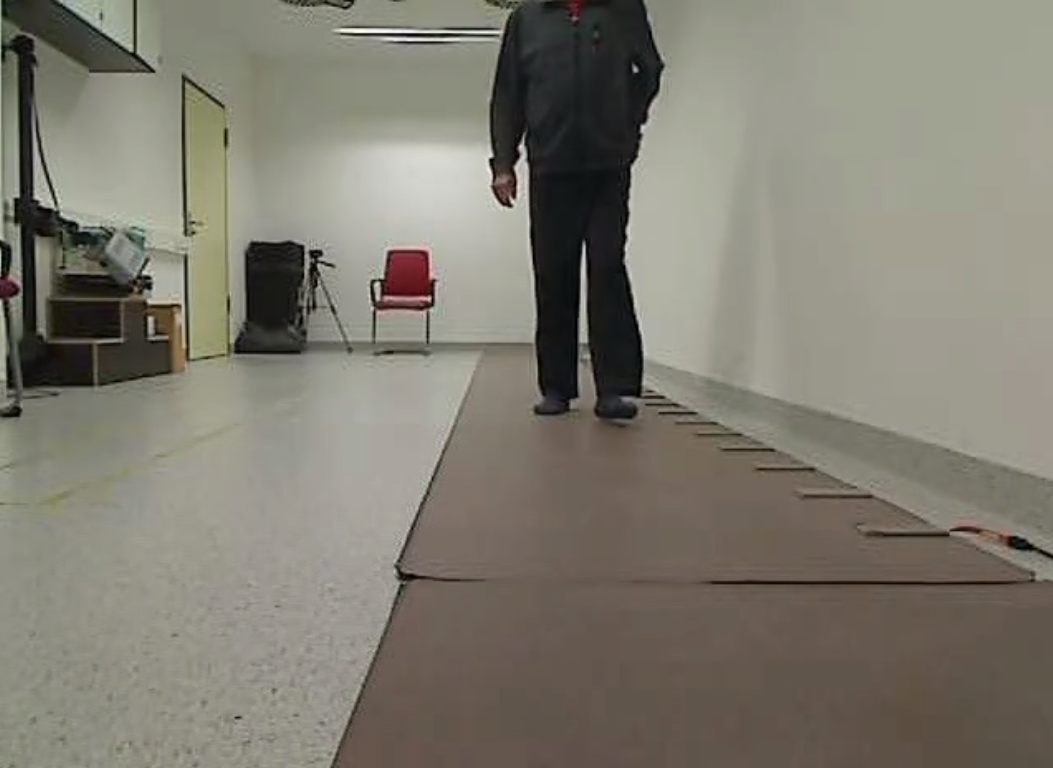
\includegraphics[width=\linewidth]{gp21.png}
    	\caption{No noise joint}
    \end{subfigure}
    \begin{subfigure}[b]{0.3\linewidth}
   		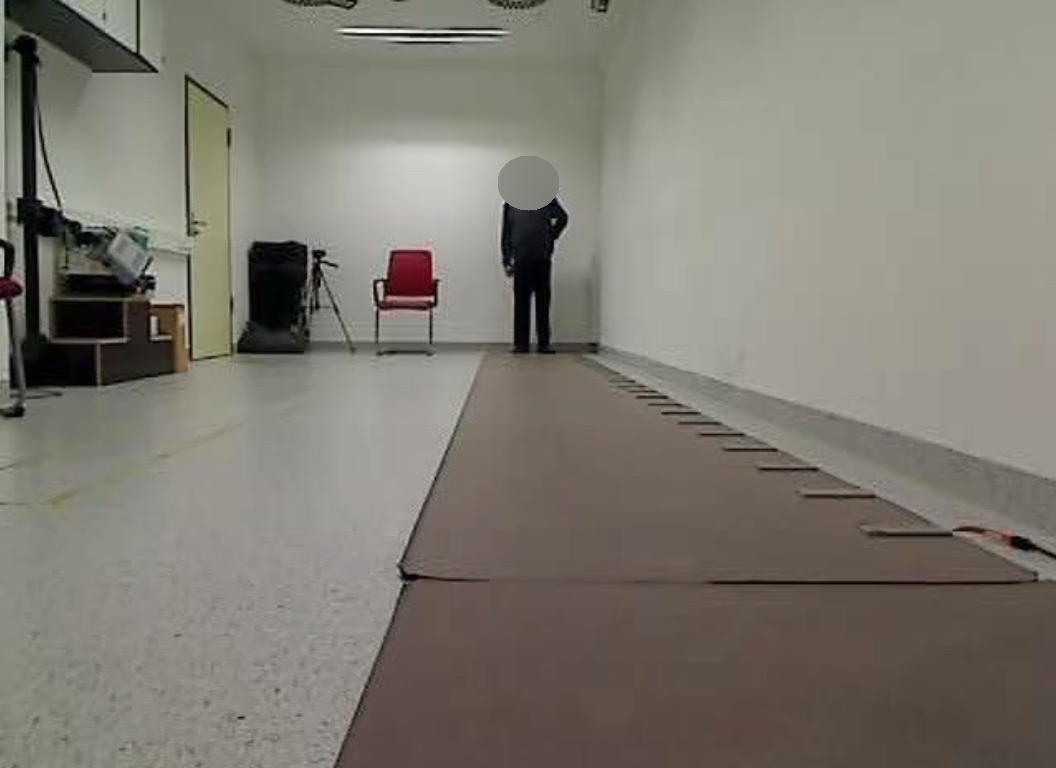
\includegraphics[width=\linewidth]{gp20.png}
    	\caption{Small apparent size}
    \end{subfigure}
    \caption{Example frames from the gait dataset illustraiting various challenging situations}
    \label{fig:gait-problems}
\end{figure}

The problem of 3D human pose estimation from monocular images is an ill-defined problem since many 3D poses can be projected to the same 2D pose. Additionally, our dataset contains many of the difficulties associated with in-the-wild scenarios. In essence we need to estimate 3D poses for arbitrary camera viewpoints and distances for a variety of body sizes given a noisy 2D inputs. On top of this we need to cope with a scene which is visually different from laboratory motion capture setup which most 3D pose datasets rely on. Moreover, the size of the data that we are coping is large when compared to other medical datasets. We have more than 77000 gait videos which need to be used for training a gait estimator. This is also a concern when we think about the time to train a model on such a large dataset.

\subsection{Scope}

We made some assumptions which limit the scope of this thesis. Firstly, we made the assumption that the existing 2D pose estimators especially open-pose from \parencite{cao2016realtime} are reliable and robust for inference in the gait dataset. Open-pose is a multi person 2D pose estimator which achieved 79.7 mAP score on the MPII dataset and 60.5 AP score on the test set of COCO 2016 keypoint challenge which are both very challenging dataset having diverse set of poses and environments. We did not have ground truth annotations for 2D pose in the gait dataset and the development of a novel 2D joint estimator was out of the scope for this thesis.

Secondly, many aspects of 3D pose estimation like pose estimation in novel viewpoints and camera distances, multi person pose estimation, pose estimation in visually challenging scenarios are examined. The improvement and extention of 3D pose estimation methods so that they work well during inference in the gait dataset was the main focus of this thesis. The 3D pose estimation is calculated relative to the root joint in our analysis. We examine the results for the absolute pose estimation case as well. However, they are not used to estimate the gait parameters.

Lastly, we did not use the Z-matrix predictions in a prediction of a diagnosis since the existing dataset had diagnosis for only a small section of the patients. Although having a diagnosis tool which gives diagnostic information from only a few gait sequences would be very beneficial, this step is out of the scope for this thesis.

\subsection{Data}

For training 3D pose estimation methods we used the Human3.6M \parencite{ionescu2014human3} and MPI-INF-3DHP \parencite{mehta2017monocular} datasets. For the gait parameter estimation we used the gait dataset.

\subsubsection{Human3.6M dataset}

Human3.6M is the largest publicly available dataset for 3D pose estimation to date. It contains 3.6 million images annotated with 2D and 3D ground truth poses. It is recorded through 4 calibrated high resolution 50 fps cameras. In addition to that the motion capture setup contains 10 different motion capture cameras and a time of flight sensor to accurately capture the motions in 3D. The motions sequences featuring 15 everyday activities including walking, smoking, and eating are performed by 7 professional actors who vary in terms of their height and body compositions. The dataset also contains additional information like high resolution body scans of the actors, camera parameters and bounding boxes for the actors. \autoref{fig:human3.6M} shows a sample of the images contained in the dataset from various viewpoints.

\begin{figure}[htpb]
    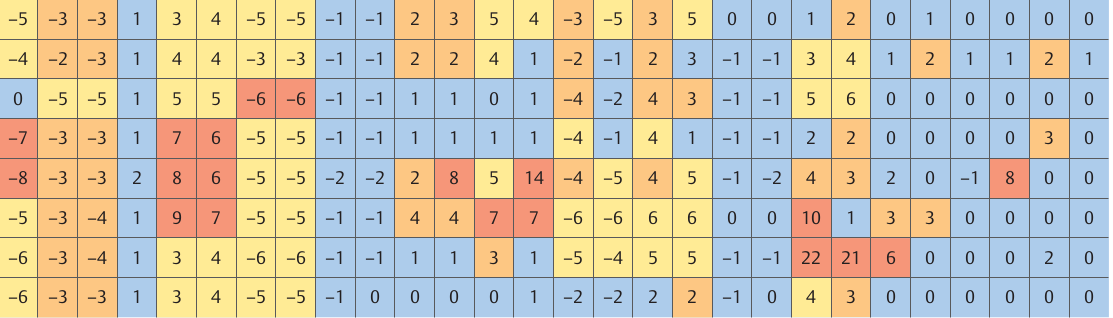
\includegraphics[width=\linewidth]{zmatrix.png}
    \caption{Examples images from the Human3.6M dataset\parencite{ionescu2014human3}}
    \label{fig:human3.6M}
\end{figure}

\subsubsection{MPI-INF-3DHP dataset}

MPI-INF-3DHP dataset although not as large as Human3.6M is also very important since it contain more challenging scenes which resemble in the wild scenarios. 8 actors are recorded performing 8 activities ranging from dynamic actions and exercises to walking and sitting. The performance is captured using 14 cameras which output in total more than 1.3M images annotated with 2D and 3D poses compatible with Human3.6M "universal" skeleton.

\subsubsection{Gait dataset}

For the gait estimation task we used the gait dataset developed in the German Center for Vertigo and Balance Disorders (DSGZ). The dataset consist of more than 77K videos with their associated mean Z-matrix values. Each video consist of a single trial of one of 7 tasks. These include self-paced walking, fast-walking, slow walking, walking with eyes closed, walking while doing a calculation, walking while doing a verbal task and walking while carrying a tray. Each task can be performed multiple times and each patient can be tested multiple times. The Z-matrix is a summary of a patients gait statistics across a test captured through a pressure carpet. Each row in the Z-matrix is the mean statistics corresponding to a certain task. Each column in that matrix contain gait statistics like mean stride length, mean stride width, mean stride frequency and so on. An example of the Z-matrix can be seen in \autoref{fig:zmatrix}

\begin{figure}[htpb]
    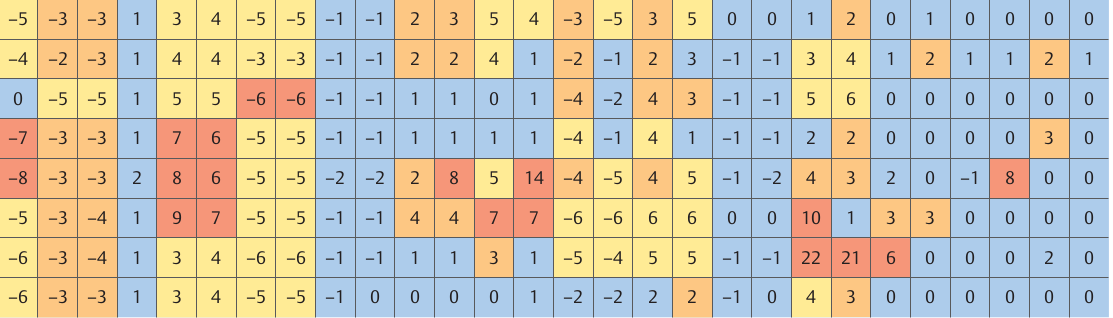
\includegraphics[width=\linewidth]{zmatrix.png}
    \caption{Visualization of the Z-matrix}
    \label{fig:zmatrix}
\end{figure}
  

The videos in the gait dataset have a resolution of 640 x 464 and are recorded at 30 fps. They are compressed with H.264 codec and 640 kbps bitrate and are on average 30 seconds long. The videos are captured from the knee height looking towards the gait carpet along the direction of the carpet. For example screen-shot please look at \autoref{fig:gait-footage}

\section{Method Outline}

This work aims at estimating the gait parameters given a monocular video of a walking person taking a gait test. The gait videos present a challenging problem given their unique set of limitations. We split the problem into 3 parts. Estimation 2D pose sequence given a monocular video, lifting 2D pose sequence to 3D and estimating gait parameters from 3D pose sequence. This division is a result of practical concerns and experimental results. Below we give a brief outline of each of the three parts.

\subsection{2D Pose Estimation}

We examine the rationale behind the decoupling of 2D and 3D pose estimations and summarize the advantages of using the open-pose \parencite{cao2016realtime} model for 2D pose estimation. We examine the pose estimation results qualitatively and show the various problems that arise from the 2D pose estimations.

\subsection{3D Pose Estimation}

We trained multiple 2D-3D pose estimators and trained them to obtain accurate 3D poses from different viewpoints and distances. The input to the model is the xy-pixel location of a set of joints and the output is 3D location of the joints in mm space.

One first model is using feed forward network with residual connections in a frame by frame basis. Our choice of network is multi layered feed forward network with residual connections \parencite{he2016deep}, dropout \parencite{srivastava2014dropout}, batch norm layer \parencite{ioffe2015batch} and max norm layer. The effect of using Rectified Linear Units (ReLU) \parencite{nair2010rectified} and Self-normalizing Linear Units (SeLU) \parencite{klambauer2017self} as the activation function for the network are compared. The 2D poses given as input may come from the ground truth or may be an output of any off the shelf 2D pose detector. The effect of normalization, taking translation in the coordinate frame to the hip joint and rotating the coordinate frame to align with the camera direction is examined. 

The second model is exploiting temporal information by using a synchronized sequence to sequence network. Long-Short-Term-Memory (LSTM) \parencite{hochreiter1997long} cells with recurrent dropout \parencite{semeniuta2016recurrent} is used as the building block. We use the synchronized sequence to sequence model since we know that each 2D pose in the sequence is corresponding to 3D pose element and the sizes of the two sequences are the same. This makes the connection pattern for the network much simpler. The LSTM blocks can fill in missing joints by tracking the movement of joints and interpolating between them. They also act as a regularizer combining information from different time steps.  

The third model is using additional height information together with a loss function which preserves the lengths of the bones. Additional information about the height helps solve the ambiguity relating to distance and size of the body. Additionally it helps the network to work for people with different body sizes and body compositions. Bone length loss helps the network estimate the length of bones and makes sure it stays constant during the sequence. 3D pose estimation is an ill-defined problem on its own however these additional priors and data help the network disambiguate challenging poses.

\subsection{Gait Assessment}

Gait assessment is done using a multi layered Bidirectional Recurrent Neural Networks \parencite{schuster1997bidirectional} which uses Long-Short-Term-Memory (LSTM) \parencite{hochreiter1997long} cells with recurrent dropout \parencite{semeniuta2016recurrent}. Each video is used to estimate one row in the Z-matrix. For the input 2D and 3D pose sequences are evaluated and compared. The problem is solved as a regression problem by estimating the size of various parameters.

\section{Thesis Organization}

The thesis organization is as follows: In chapter 2 we review the the related literature. This chapter discusses different approaches for 2D and 3D human pose estimation and summarize them. In chapter 3 we examine the 2D pose estimation model and its performance in the gait dataset. In chapter 4, we examine various 3D pose estimation models, including a feed forward network with residual connections, a synchronized sequence to sequence network. Additionally, we examine the effect of viewpoint augmentation, data representation techniques, data normalization, different loss function like bone length loss and additional datasets. In chapter 5 we examine the problem of gait parameter estimation given 2D and 3D pose sequences. Finally in chapter 6, we highlight our main contributions and discuss possible future directions. 